\section{Dataset overview}
\label{sec:dataset}

\begin{figure}
    \centering
    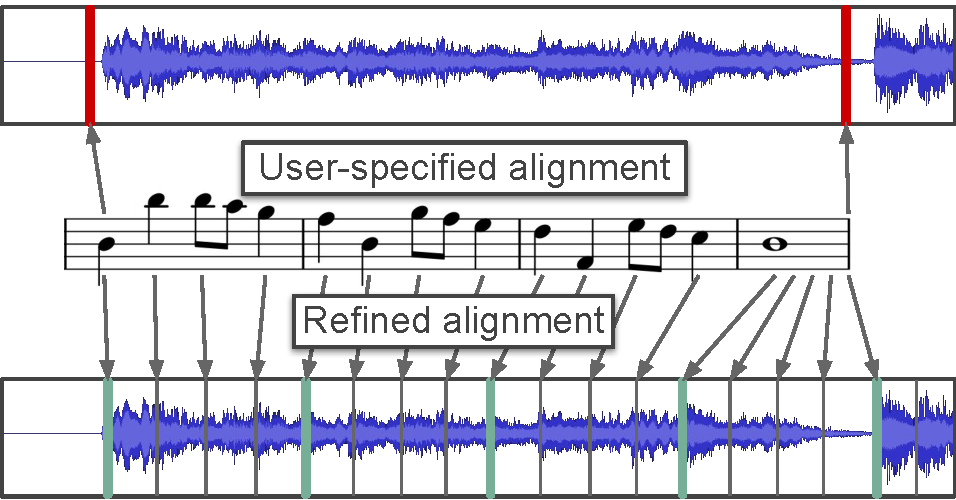
\includegraphics[width=8.1cm]{figs/alignment.pdf}
    \caption{We refine coarse, user-specified alignments from \hooktheory{} by using beat tracking. The first segment beat is mapped to the detected downbeat nearest to the user-specified starting timestamp, and remaining beats are mapped to subsequent detected beats.}
 \label{fig:alignment}
\end{figure}

We collect and release a dataset of crowdsourced melody and chord annotations from \hooktheory{}. 
The dataset comprises annotations for $22$k segments of $13$k unique recordings---together, these segments comprise $50$ hours of labeled audio. 
The audio content covers a wide range of genres---there is a skew towards pop and rock but many other genres are represented including EDM, jazz, and even classical. 
We create an artist-stratified $8$:$1$:$1$ split of the dataset for training, validation, and testing.

\todo{Copied from intro. Need to integrate}
While data from \hooktheory{} has been used previously for tasks like harmonization~\cite{chen2021surprisenet,yeh2021automatic}, chord recognition~\cite{jiang2019mirex}, and representation learning~\cite{jiang2020transformer}, making use of this platform for MIR is currently cumbersome and involves web scraping, reverse engineering a proprietary score format, and audio-to-score alignment. 
To ease this burden, we release all of the annotations in a simplified MIDI-like format under a Creative Commons license, with links and alignments to the audio on YouTube. 

\hooktheory{} users annotate the audio in a proprietary ``functional'' format, i.e., one which uses scale degrees and roman numerals relative to a key signature instead of absolute notes and chord names. 
Absolute labels are used by the vast majority of transcription work---hence, we convert this proprietary functional format into a simple absolute one. 
Note that users annotate melodies with only relative octave information, i.e.,~intervals between melody notes should be accurate, but the absolute octave of the melody may be incorrect relative to the recording.

\subsection{Alignment}

With the release of this dataset, we also make an effort to improve the alignments between the annotations and the audio. 
By default, users provide only a coarse audio alignment, specifying the starting and ending timestamps of the annotated segment. 
These alignments are overall poor---the starting/ending timestamps are often sloppy, and any tempo fluctuations within a segment will further jeopardize the alignment.

We use the beat and downbeat detection algorithm from \madmom{}~\cite{bock2016joint,bock2016madmom} to refine these alignments. 
Our approach aligns the first beat of the segment to the detected downbeat which is nearest to the user-specified starting timestamp. 
Then, we align the remaining beats to the subsequent consecutive detected beats (see~\Cref{fig:alignment} for an example). 
This provides a beat-level alignment for the entire segment, and we use linear interpolation for fractional beat subdivisions. 
In an informal listening test, this produces an excellent alignment in around $95\%$ of cases, where the primary failure mode in the remaining $5\%$ occurs when \madmom{} detects the wrong beat as the downbeat. 
We use these refined alignments for training and evaluation, accepting the glitched alignments as noise in the dataset.